\documentclass{beamer}

% Theme 
% \usetheme{Warsaw}
\usetheme{Frankfurt}
\setbeamertemplate{page number in head/foot}[totalframenumber]

\usepackage{graphicx}
\usepackage{amsmath}
\usepackage{amsfonts}
\usepackage{amssymb}
\usepackage{tikz}
\usetikzlibrary{calc}

\usepackage{listings}
\usepackage{xcolor}

\usepackage{hyperref}

\hypersetup {
    colorlinks=true,
    linkcolor=blue,
    urlcolor=blue
}

\lstdefinestyle{python}{
    language=Python,
    basicstyle=\ttfamily\small,
    keywordstyle=\color{blue},
    commentstyle=\color{red},
    stringstyle=\color{green},
    breaklines=true,
    breakatwhitespace=true,
    tabsize=4
}

\title{Latent Diffusion Models}
\author[Nathan Van Maastricht]{Nathan Van Maastricht}

\begin{document}
\begin{frame}
    \titlepage
\end{frame}

\section{Diffusion}
\begin{frame}
    \frametitle{Diffusion}
    \begin{block}{Diffusion}
        Generative diffusion is the process of learning to reverse entropy
    \end{block}

    \begin{block}{}
        We literally take random noise and turn it into coherent data
    \end{block}
\end{frame}

\begin{frame}
    \frametitle{Physical Diffusion}
    \begin{block}{Mechanism}
        Spontaneous movement of particles from regions of high concentration to low concentration
    \end{block}
    
    \begin{block}{Generative Approach}
        If we can precisely model the local drift that causes this dispersion, we can mathematically invert time to recover structure from the chaos
    \end{block}
\end{frame}

\begin{frame}
    \frametitle{Physical Diffusion}
    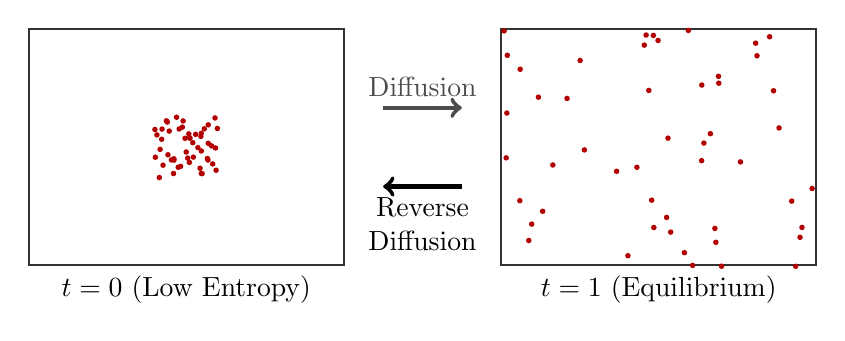
\begin{tikzpicture}[
        particle/.style={circle, fill=red!70!black, minimum size=2pt, inner sep=0pt},
        box/.style={draw=black!80, thick, minimum width=4cm, minimum height=3cm}
    ]

    % Pane 1: Low Entropy (t=0)
    \node[box, label=below:{$t=0$ (Low Entropy)}] (box1) at (0,0) {};
    \foreach \i in {1,...,50} {
        \node[particle] at ([shift={(rand*0.4, rand*0.4)}]box1.center) {};
    }

    % Arrow
    \draw[->, ultra thick, black!70] (2.5,0.5) -- (3.5,0.5) node[midway, above] {Diffusion};

    \draw[->, ultra thick, black!100] (3.5, -0.5) -- (2.5, -0.5) node[midway, below, align=center] {Reverse \\ Diffusion};

    % Pane 2: High Entropy (t=T)
    \node[box, label=below:{$t=1$ (Equilibrium)}] (box2) at (6,0) {};
    \foreach \i in {1,...,50} {
        % Distribute randomly across the whole box
        \node[particle] at ($(box2.south west) + (4*rnd, 3*rnd)$) {};
    }

    \end{tikzpicture}
\end{frame}

\begin{frame}
    \frametitle{Flow Matching}
    Define a time dependent vector field $v_t(x)$ that describes the velocity of a smple moving from a simple distribution (such as Gaussian nosie) to the complex data distribution (such as real images). This is encoded in the relatively basic looking ODE $$\frac{dx}{dt}=v_t(x)$$

    \begin{block}{Learning Objective}
        We learn this velocity field directly.
    \end{block}
\end{frame}

\begin{frame}
    \begin{columns}[c]
        \begin{column}{0.5\textwidth}
            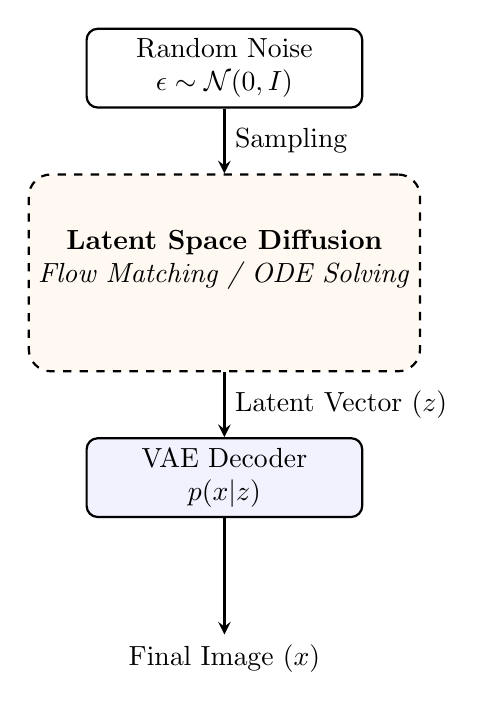
\begin{tikzpicture}[
                node distance=1.8cm, 
                auto, 
                >=stealth, 
                thick,
                box/.style={draw, rectangle, minimum width=3.5cm, minimum height=1cm, align=center, rounded corners=4pt},
                latent/.style={draw, rectangle, fill=orange!5, minimum width=4cm, minimum height=2.5cm, align=center, dashed, rounded corners=8pt},
                arrow/.style={->, line width=1pt}
            ]

                % Top: Starting Point
                \node [box] (noise) {Random Noise \\ $\epsilon \sim \mathcal{N}(0, I)$};
                
                % Middle: The "Engine"
                \node [latent, below of=noise, yshift=-0.8cm] (process) {
                    \textbf{Latent Space Diffusion} \\ 
                    \textit{Flow Matching / ODE Solving} \\
                    % \vspace{0.5cm}
                };
                
                % Bottom: The Reconstruction
                \node [box, fill=blue!5, below of=process, yshift=-0.8cm] (decoder) {VAE Decoder \\ $p(x|z)$};
                
                % Final Output
                \node [below of=decoder, yshift=-0.5cm] (image) {Final Image ($x$)};

                % Connecting Arrows
                \draw [arrow] (noise) -- (process) node[midway, right] {Sampling};
                \draw [arrow] (process) -- (decoder) node[midway, right] {Latent Vector ($z$)};
                \draw [arrow] (decoder) -- (image);

                % Small Vector Field Graphic inside the Latent box
                % \begin{scope}[shift={($(process.center)+(0,-0.3)$)}]
                %     \foreach \x in {-1.2, -0.4, 0.4, 1.2}
                %         \foreach \y in {-0.2, 0.3}
                %             \draw[->, gray!60, thin] (\x,\y) -- +({0.2*cos(45)}, {0.2*sin(45)});
                % \end{scope}

            \end{tikzpicture}
        \end{column}

        \begin{column}{0.5\textwidth}
            \centering
            
\includegraphics[width=5cm]{images/rnd_latent.png}
            \vspace{3cm}

            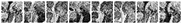
\includegraphics[width=5cm]{images/final_latent.png}
            \vspace{1cm}

            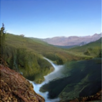
\includegraphics[width=2.5cm]{images/output_image.png}
        \end{column}
    \end{columns}
\end{frame}

\begin{frame}
    \frametitle{Data}
    \begin{itemize}
        \setlength{\itemsep}{1em}
        \item CC12M is a dataset composed by google, with roughly 6M image/caption pairs still available
        \item Re-LAION-Caption 19M is by supermodel research derived from LAION 5B, using roughly 3M images, with four potential captions each, focusing on subject, setting, aesthetic, camera details
    \end{itemize}
\end{frame}

\section{VAE}

\begin{frame}
    \frametitle{The VAE's Job}
    \begin{enumerate}
        \setlength{\itemsep}{1em}
        \item Encode images to latents
        \item Decode latents to images
        \item Structure the latent space so a diffusion model can learn how it is structured
    \end{enumerate}
\end{frame}

\begin{frame}
    \frametitle{VAE Architecture}
    \begin{itemize}
        \setlength{\itemsep}{1em}
        \item Residual Blocks
        \item Attention Blocks
        \item Upsampling Blocks
        \item Downsampling Blocks
        \item FSQ Layer
    \end{itemize}
\end{frame}

\begin{frame}[fragile]
    \frametitle{Residual Blocks}
    \begin{itemize}
        \setlength{\itemsep}{1em}
        \item Preactivation style (normalise and activation first)
        \item Additive residuals (add rather than concatenate)
    \end{itemize}

\begin{center}
\begin{lstlisting}
h = self.conv1(self.act(self.norm1(x)))
h = self.conv2(self.act(self.norm2(h)))

return h + self.shortcut(x)
\end{lstlisting}
\end{center}
\end{frame}

\begin{frame}[fragile]
    \frametitle{Attention Blocks}
    \begin{itemize}
        \setlength{\itemsep}{1em}
        \item Global Context
        \item Flash Attention 2 for fast attention kernels
    \end{itemize}

    \begin{center}
\begin{lstlisting}
qkv = self.qkv(self.norm(x))
q, k, v = torch.chunk(qkv, 3, dim=1)

out = F.scaled_dot_product_attention(
    q, k, v, 
    dropout_p=self.dropout, 
    scale=self.scale
)

return x + self.proj_out(out)
\end{lstlisting}
    \end{center}
\end{frame}

\begin{frame}
    \frametitle{Spatial Resizing}
    \begin{itemize}
        \setlength{\itemsep}{1em}
        \item \textbf{Downsampling:} Uses a convolutional layer with a $3\times 3$ kernel and a stride of 2 to reduce the spatial dimensions by half
        \item \textbf{Upsampling:} Uses nearest neighbour interpolation to upscale the spatial dimensions by a factor of 2, followed by a convolutional layer to reduce checkerboard artifacting that appears with transposed convolutions
    \end{itemize}

    The downsampling block and upsampling block are attempting to be mirror images of each other with respect to the spatial dimensions
\end{frame}

\begin{frame}
    \frametitle{FSQ Layer}
    \begin{itemize}
        \setlength{\itemsep}{1em}
        \item Map continuous latents to a discrete grid
        \item Use a scaled sigmoid ($2\sigma(1.6x)-1$) to squash values into $[-1,1]$
        \item Round values to fixed levels, in my case 15 levels per dimension
        \item Use a straight through estimator to bypass the non-differentiable rounding function
    \end{itemize}
\end{frame}

\begin{frame}
    \frametitle{Why FSQ-VAE?}
    \begin{itemize}
        \setlength{\itemsep}{1em}
        \item No codebook collapse: Standard VQ-VAE have dead entries that never get used because the codebook is learned. In an FSQ-VAE the levels are predefined
        \item The straight through estimator passes the correct quantised latent to the decoder, and the correct gradients back to the encoder, while going through a non differentiable function. Very similar to the reparameterisation trick in a KL-VAE
    \end{itemize}
\end{frame}

\begin{frame}
    \frametitle{Why $2\sigma(1.6x)-1$?}
    \centering
    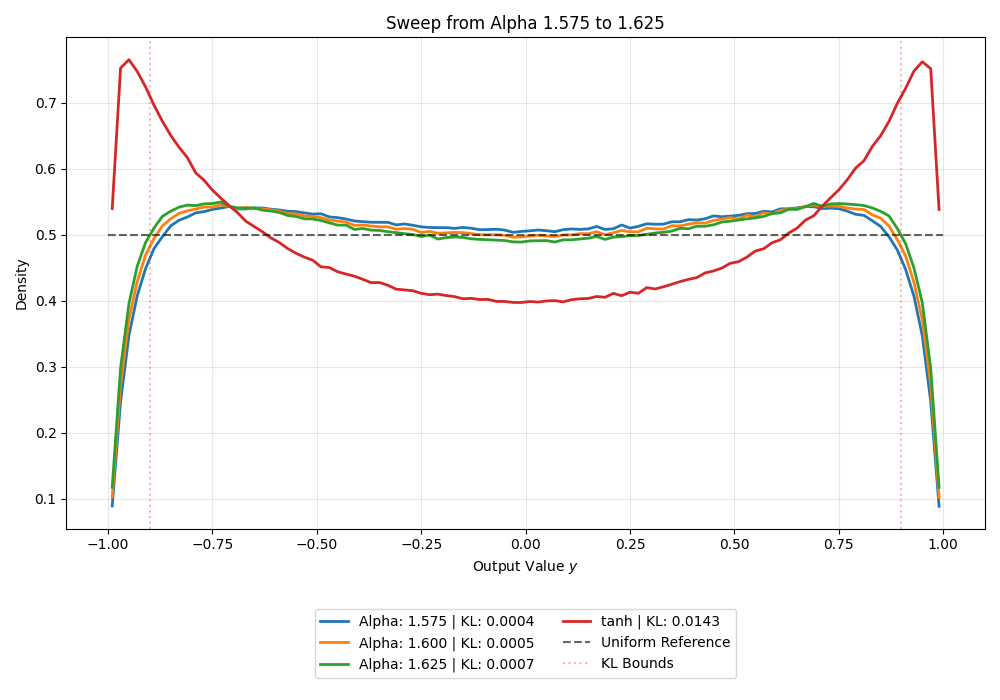
\includegraphics[width=0.9\textwidth]{images/range_based_sweep.png}
\end{frame}

\begin{frame}
    \frametitle{VAE Summary}
    \begin{itemize}
        \setlength{\itemsep}{1em}
        \item Model type: FSQ-VAE
        \item Input Resolution: $256\times256\times3$
        \item Quantised Grid: $[15, 15, 15, 15, 15, 15, 15, 15]$
        \item Codebook size: $15^8$
        \item Downsampling Factor: $8\times (256\rightarrow32)$
        \item Compression Factor: $24\times$. $256\times256\times3$ $(196,608) \rightarrow 32\times32\times8$ $(8,192)$
    \end{itemize}
\end{frame}

\begin{frame}
    \frametitle{Training the VAE: Loss}
    \begin{itemize}
        \setlength{\itemsep}{1em}
        \item Reconstruction: L1 measures pixel-wise fidelity, ensuring the global structure is correct. Often leads to blurriness if the only component of the loss.
        \item Adversarial: A discriminator model is fed the original image and reconstructed image. The VAE wants to fool the discriminator, which pushes it to produce sharper images.
        \item Feature Matching: Using the same discriminator model, compare the internal activations for the real and fake images to ensure statistical and perceptual features match.
    \end{itemize}
\end{frame}

\begin{frame}
    \frametitle{Training the VAE: Warmup and Cooldown}
    \begin{itemize}
        \setlength{\itemsep}{1em}
        \item Adversarial Warmup: The adversarial component of the loss function linearly grows to a maximum value, allowing the VAE to partially learn reconstruction before being pushed by the discriminator to shape the latent space appropriately. This is roughly 10\% of the training time
        \item Learning Rate: The learning rate starts at roughly 10\% of it's maximum rate, and linearly grows over the first 10\% of training. Then it is held at this maximum rate until the last 10\% of it's training, where it decays along a cosine curve, allowing the model to fall deep into the local minimum it has found
    \end{itemize}
\end{frame}

\begin{frame}
    \frametitle{VAE Training Visualisations}
    \centering
    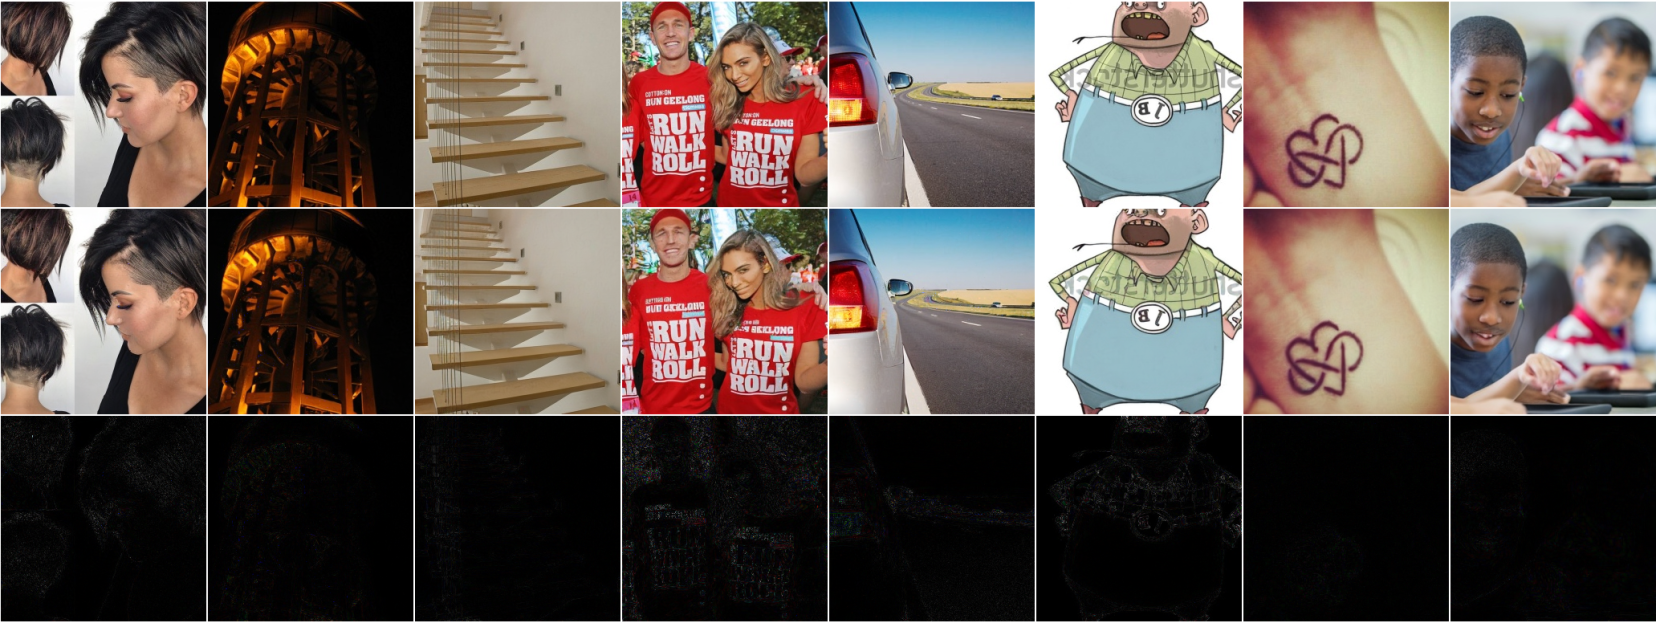
\includegraphics[width=\textwidth]{images/final_vae.png}
\end{frame}

\begin{frame}
    \frametitle{VAE: What's Been Skipped?}
    \begin{itemize}
        \setlength{\itemsep}{1em}
        \item Code book utilisation monitoring
        \item Program optimisation such as memory management, device management
        \item Training compromises such as gradient accumulation, what effective batch size is useful, how hyperparameter values were selected, why some values had warmup and some didn't
        \item Any details on the discriminator at all, for example why use spectral normalisation
        \item Gradient clipping
    \end{itemize}
\end{frame}

\section{DiT-UNet}

\begin{frame}
    \frametitle{Training DiT-UNet}
    \begin{itemize}
        \setlength{\itemsep}{1em}
        \item The VAE encodes images into latents
        \item Noise is added to the latents proportional to a time variable between 0 and 1
        \item The DiT-UNet predicts a proxy for this noise called ``velocity''
    \end{itemize}
\end{frame}

\begin{frame}
    \frametitle{Architecture}
    \begin{itemize}
        \setlength{\itemsep}{1em}
        \item 16 Transformer blocks using patch-based attention
        \item Skip connections link early blocks to late blocks
        \item Self-attention to capture spatial dependencies
        \item Cross-attention to inject text conditioning
    \end{itemize}
\end{frame}

\begin{frame}[fragile]
    \begin{center}
        \resizebox{\textwidth}{!}{
            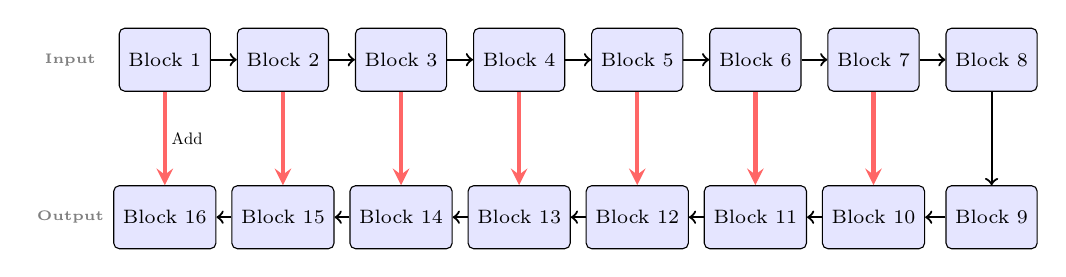
\begin{tikzpicture}[
                node distance=1.5cm,
                block/.style={draw, fill=blue!10, minimum width=1.1cm, minimum height=0.8cm, rounded corners=2pt, font=\scriptsize, align=center},
                io/.style={font=\tiny\bfseries, gray},
                skip/.style={->, red!60, ultra thick, >=stealth},
            ]
                % Top Row: Encoder
                \node [block] (b1) {Block 1};
                \node [block, right of=b1] (b2) {Block 2};
                \node [block, right of=b2] (b3) {Block 3};
                \node [block, right of=b3] (b4) {Block 4};
                \node [block, right of=b4] (b5) {Block 5};
                \node [block, right of=b5] (b6) {Block 6};
                \node [block, right of=b6] (b7) {Block 7};
                \node [block, right of=b7] (b8) {Block 8};

                % Bottom Row: Decoder (Aligned under Encoder)
                \node [block, below of=b8, yshift=-0.5cm] (b9) {Block 9};
                \node [block, left of=b9] (b10) {Block 10};
                \node [block, left of=b10] (b11) {Block 11};
                \node [block, left of=b11] (b12) {Block 12};
                \node [block, left of=b12] (b13) {Block 13};
                \node [block, left of=b13] (b14) {Block 14};
                \node [block, left of=b14] (b15) {Block 15};
                \node [block, left of=b15] (b16) {Block 16};

                % Flow Arrows
                \draw [->, thick] (b1) -- (b2);
                \draw [->, thick] (b2) -- (b3);
                \draw [->, thick] (b3) -- (b4);
                \draw [->, thick] (b4) -- (b5);
                \draw [->, thick] (b5) -- (b6);
                \draw [->, thick] (b6) -- (b7);
                \draw [->, thick] (b7) -- (b8);
                \draw [->, thick] (b8) -- (b9); % The "Turn"
                \draw [->, thick] (b9) -- (b10);
                \draw [->, thick] (b10) -- (b11);
                \draw [->, thick] (b11) -- (b12);
                \draw [->, thick] (b12) -- (b13);
                \draw [->, thick] (b13) -- (b14);
                \draw [->, thick] (b14) -- (b15);
                \draw [->, thick] (b15) -- (b16);

                % Skip Connections (Vertical)
                \draw [skip] (b1) -- (b16) node[midway, right, black, scale=0.6] {Add};
                \draw [skip] (b2) -- (b15);
                \draw [skip] (b3) -- (b14);
                \draw [skip] (b4) -- (b13);
                \draw [skip] (b5) -- (b12);
                \draw [skip] (b6) -- (b11);
                \draw [skip] (b7) -- (b10);

                % Input/Output labels
                \node [left of=b1, xshift=0.3cm, io] {Input};
                \node [left of=b16, xshift=0.3cm, io] {Output};

            \end{tikzpicture}
        }
    \end{center}
\end{frame}

\begin{frame}
    \frametitle{Attention}
    \begin{itemize}
        \setlength{\itemsep}{1em}
        \item Latent tokens (patches) are related to each other by self-attention, with 2D RoPE for relative spatial relationships
        \item Mapping text tokens to spatial regions is done with cross-attention
    \end{itemize}
\end{frame}

\begin{frame}
    \frametitle{Adaptive Layer Norm}
    Instead of a static Layer Norm $\gamma$, $\beta$, and $\alpha$ are calculated per transformer block from the combined time and text embedding.

    \vspace{5mm}
    These are used in a gating mechanism, allowing less or more weight for the transformers text parameters, initially not even using the transformers parameters related to text embeddings.
\end{frame}

\begin{frame}
    \frametitle{Preprocessing}
    \begin{itemize}
        \setlength{\itemsep}{1em}
        \item Encode all images and captions ahead of time
        \item Ensure dataloader has enough bandwidth on storage to keep the compute saturated
    \end{itemize}
\end{frame}

\begin{frame}[fragile]
    \frametitle{Training the DiT-UNet}
    To recap, we're trying to train a model to learn the vector field $v_t(x)$ that satisfies $$\frac{dx}{dt}=v_t(x)$$ which corresponds to learning a straight line path from the noise $p_1$ to the data $p_0$.

    \begin{center}
    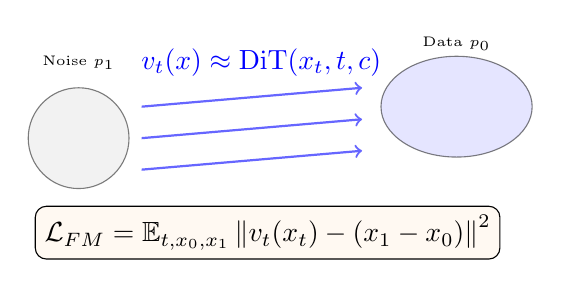
\begin{tikzpicture}[scale=0.8]
        % Noise Distribution
        \draw[fill=gray!20, opacity=0.5] (-3,0) circle (0.8);
        \node at (-3,1.2) {\tiny Noise $p_1$};
        
        % Data Distribution
        \draw[fill=blue!20, opacity=0.5] (3,0.5) ellipse (1.2 and 0.8);
        \node at (3,1.5) {\tiny Data $p_0$};
        
        % Vector Field Arrows
        \foreach \y in {-0.5, 0, 0.5} {
            \draw[->, thick, blue!60] (-2, \y) -- (1.5, \y + 0.3);
        }
        
        \node[blue] at (-0.1, 1.2) {$v_t(x) \approx \text{DiT}(x_t, t, c)$};
        
        % Equation
        \node at (0, -1.5) [draw, rounded corners, fill=orange!5] 
            {$\mathcal{L}_{FM} = \mathbb{E}_{t, x_0, x_1} \left\| v_t(x_t) - (x_1 - x_0) \right\|^2$};
    \end{tikzpicture}
    \end{center}
\end{frame}

\begin{frame}
    \frametitle{Optimisations and Stability}
    \begin{itemize}
        \setlength{\itemsep}{1em}
        \item EMA smooths out the weight updates
        \item Training in bf16 is sufficient for most calculations, with the loss being calculated in full precision still
        \item Learning rate warmup, hold, and cooldown
        \item Classifier free guidance
    \end{itemize}
\end{frame}

\begin{frame}
    \frametitle{DiT: What's been skipped?}
    \begin{itemize}
        \setlength{\itemsep}{1em}
        \item How to implement the attention mechanism, in particular how to normalise the QKV tensors
        \item Why we only apply RoPE to the self-attention but not the cross-attention
        \item Why this differential equation?
        \item Why predict the proxy rather than noise directly?
        \item Issues with data handling
        \item What's being monitored
        \item Gradient clipping
    \end{itemize}
\end{frame}

\section{Sampling}

\begin{frame}
    \frametitle{We've got a model, now what? RK2}
    \begin{enumerate}
        \setlength{\itemsep}{1em}
        \item Take a half-step using the initial velocity predicted by the model
        \item Re-evaluate the velocity field at that midpoint
        \item Take the full step using the refined velocity
    \end{enumerate}

    \begin{center}
    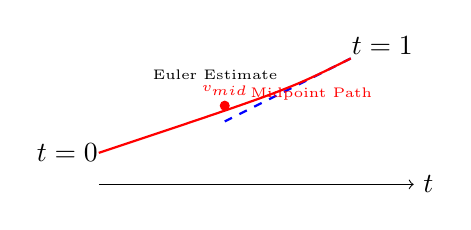
\begin{tikzpicture}[scale=0.8]
        \draw[->] (0,0) -- (5,0) node[right] {$t$};
        \draw[thick, blue, dashed] (4,2) -- (2,1) node[midway, above left, black] {\tiny Euler Estimate};
        \draw[thick, red] (4,2) .. controls (3,1.5) .. (0,0.5) node[near start, below] {\tiny Midpoint Path};
        \filldraw [red] (2,1.25) circle (2pt) node[above] {\tiny $v_{mid}$};
        \node at (4.5, 2.2) {$t=1$};
        \node at (-0.5, 0.5) {$t=0$};
    \end{tikzpicture}
    \end{center}
\end{frame}

\begin{frame}
    \frametitle{Classifier-Free Guidance}
    Classifier-Free Guidance moves the sample away from the ``generic'' distribution and toward the specific ``text-aligned'' distribution, attempting to focus the model.

    \vspace{5mm}
    There is also the concept of a negative prompt, pushing away from concepts such as ``blurred'' or ``out of focus''.
\end{frame}

\begin{frame}
    \frametitle{Post Sampling}
    \begin{itemize}
        \setlength{\itemsep}{1em}
        \item Unnormalise from DiT-UNet to VAE decoder
        \item FSQ Snapping: Round the output of the DiT to the level the FSQ-VAE expect
    \end{itemize}
\end{frame}

\begin{frame}
    \frametitle{Sample}
    \centering
    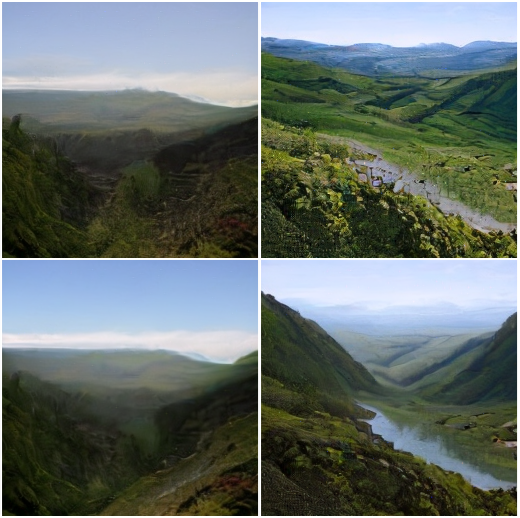
\includegraphics[height=0.8\textheight]{images/cfg_snapping.png}
\end{frame}

\begin{frame}
    \frametitle{What's been skipped?}
    \begin{itemize}
        % \setlength{\itemsep}{0.75em}
        \item Signals to watch for throughout training?
        \item How to train the language model that is being used to inject the prompts?
        \item How to determine what a ``generic'' distribution is?
        \item How to normalise and unnormalise the data at the various stages of training
        \item Guard rails
        \item How long should training go for?
        \item How to determine any of this the hyperparameters?
        \item References? Where did I learn this?
        \item Alternatives? What do the big companies do that I don't have the resources for? How do the big companies differ to each other? Who even thought this was reasonable to try?
        \item Beside pictures, where can this be used?
    \end{itemize}
\end{frame}

\begin{frame}
    \frametitle{Mid-training}
    \centering
    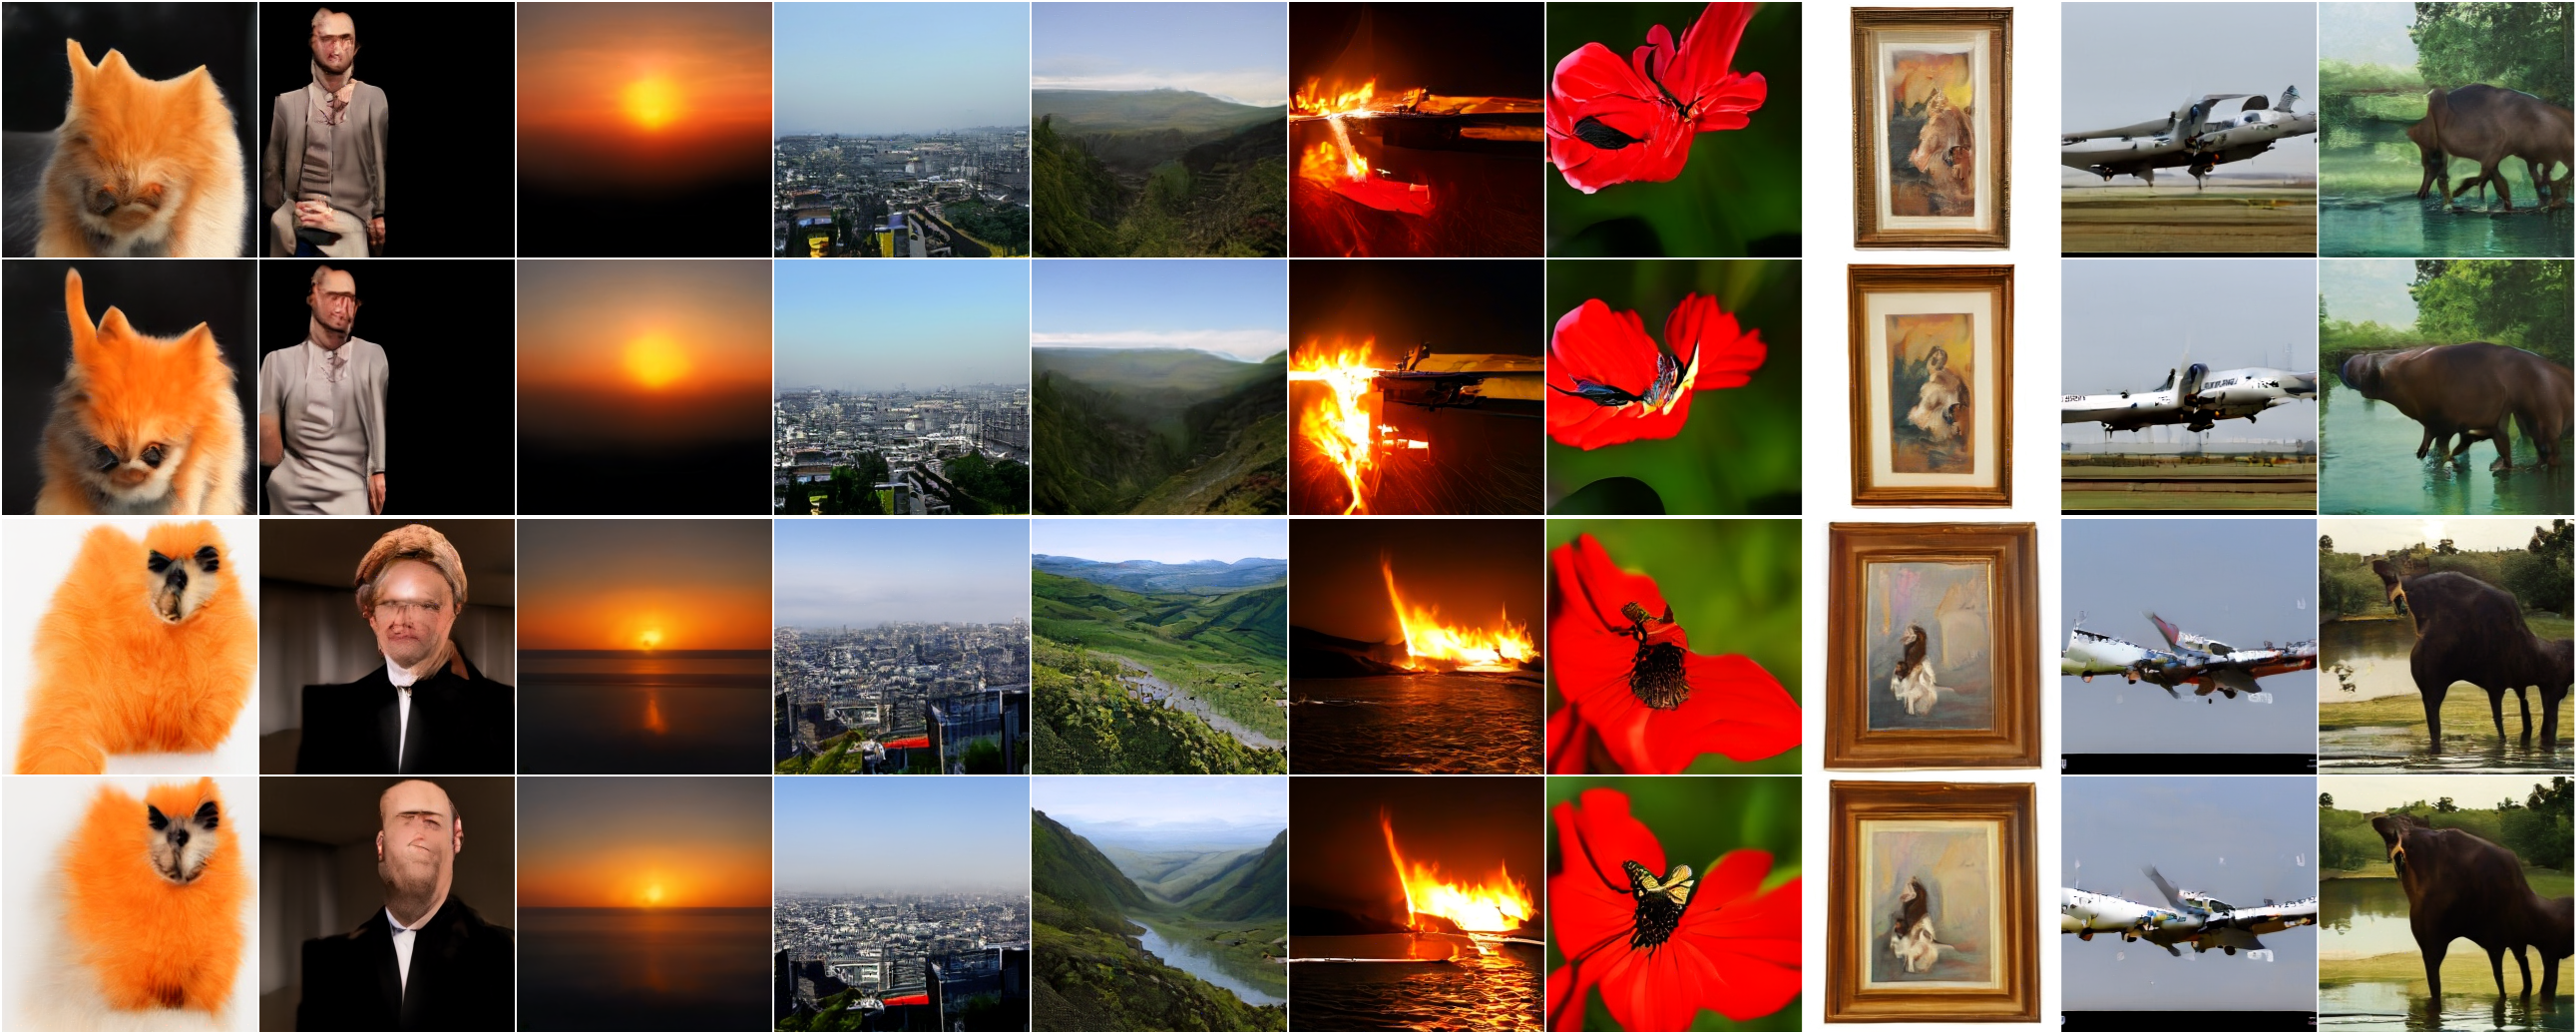
\includegraphics[width=\textwidth]{images/mid_training.png}
\end{frame}

\begin{frame}
    \frametitle{Magic?}

    \centering
    
\includegraphics[width=\textwidth]{images/rnd_latent.png}

    \vspace{2cm}
    \centering
    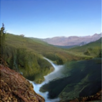
\includegraphics[height=3cm]{images/output_image.png}
\end{frame}

\end{document}